\documentclass[]{article}

\usepackage{mathtools}
\usepackage{listings}
\usepackage{clrscode}
\usepackage{algorithm}
\usepackage{algorithmic}
\usepackage{graphicx}
\usepackage[top=2cm, bottom=2cm, left=2cm, right=2cm]{geometry}
\DeclareMathOperator*{\argmin}{arg\,min}
\DeclareMathOperator*{\argmax}{arg\,max}

\title{Homework 5}
\date{2015-12-26}
\author{Jingwei Zhang 201528013229095}

\begin{document}
    \maketitle
    \section{Problem 1}
    \begin{figure}[H]
        \centering
        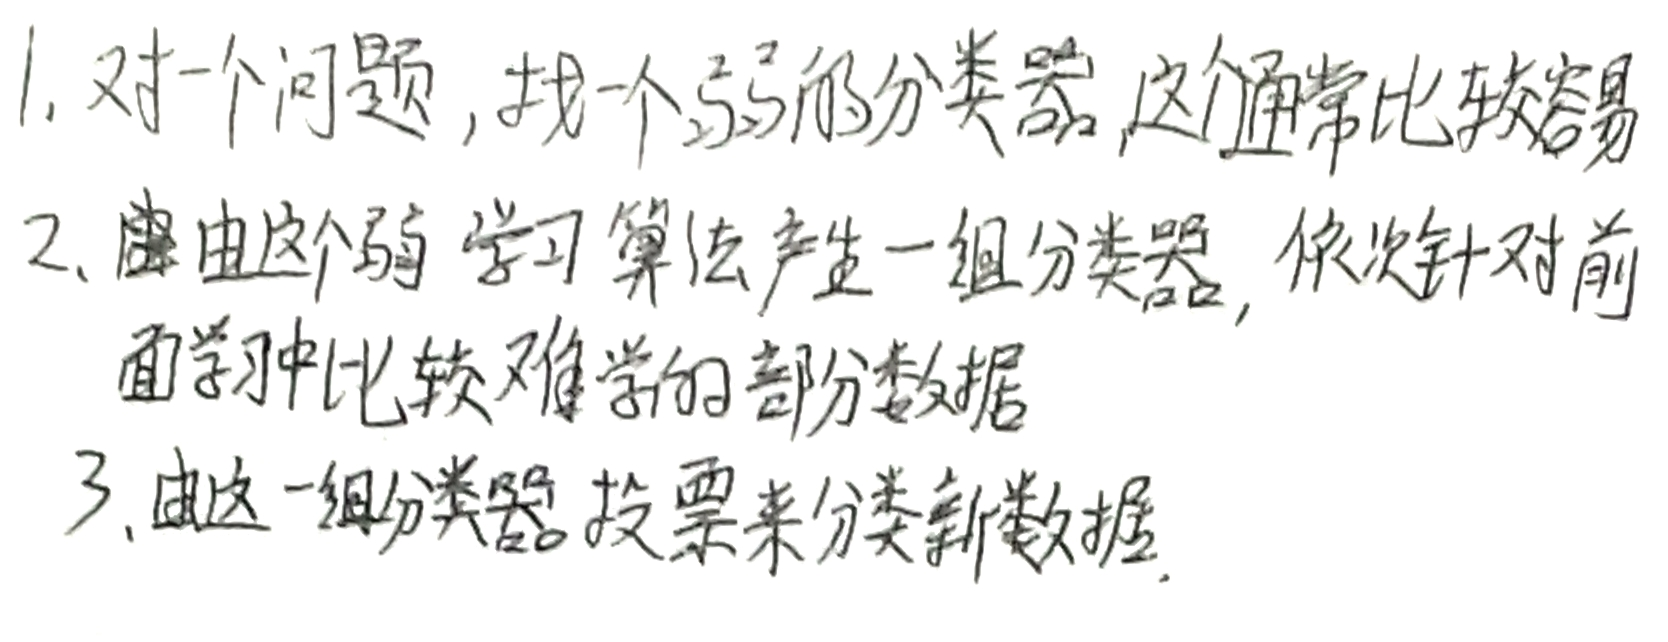
\includegraphics[scale=0.5]{P1.jpg}
    \end{figure}
    \section{Problem 2}
    \begin{figure}[H]
        \centering
        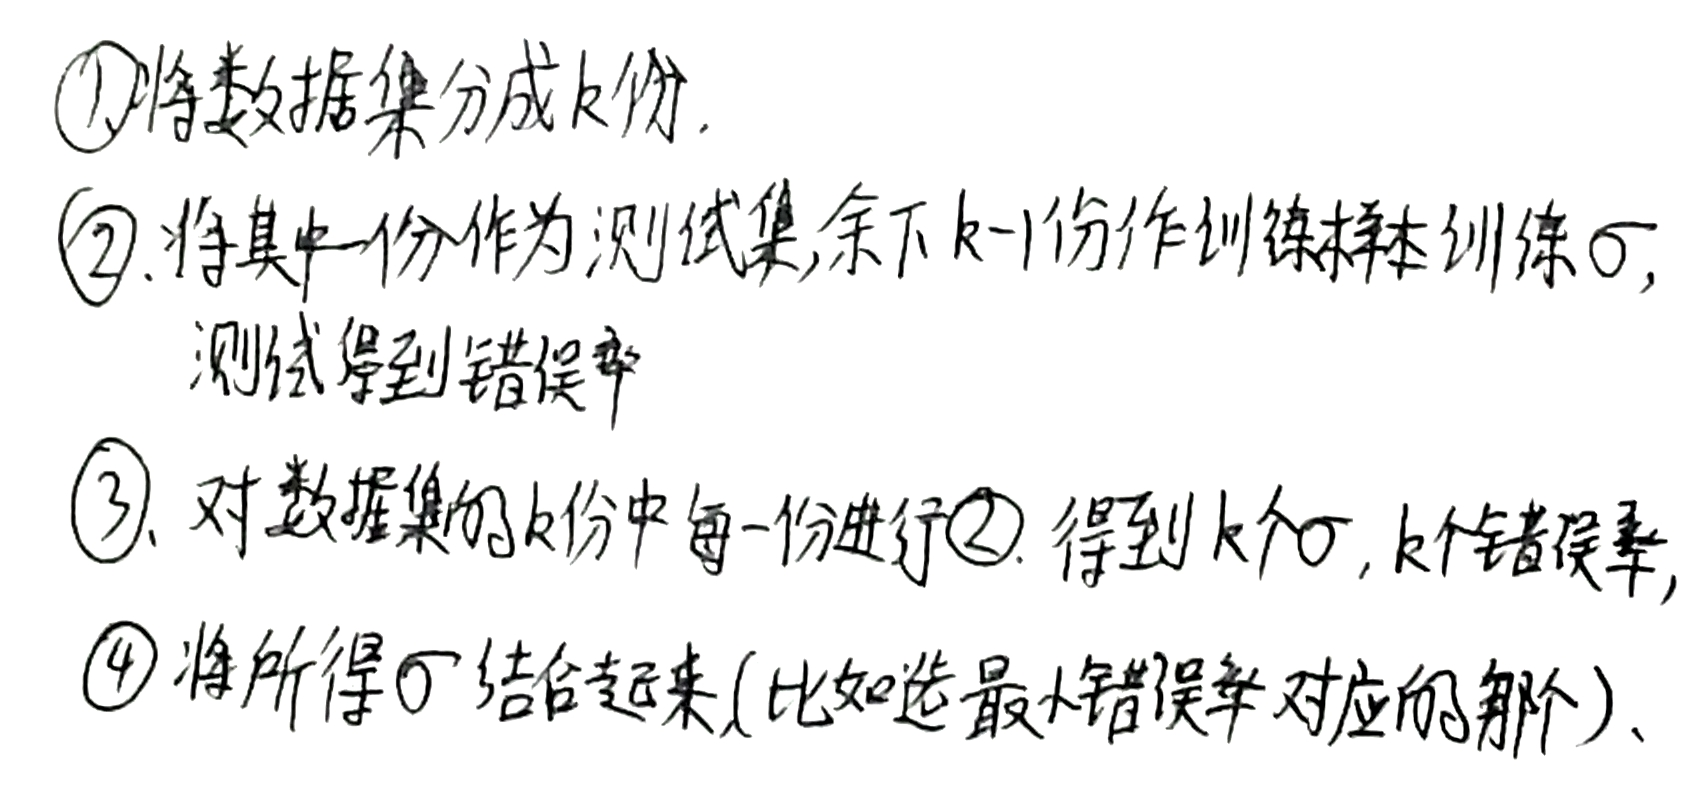
\includegraphics[scale=0.5]{P2.jpg}
    \end{figure}
    \section{Problem 3}
    \begin{figure}[H]
        \centering
        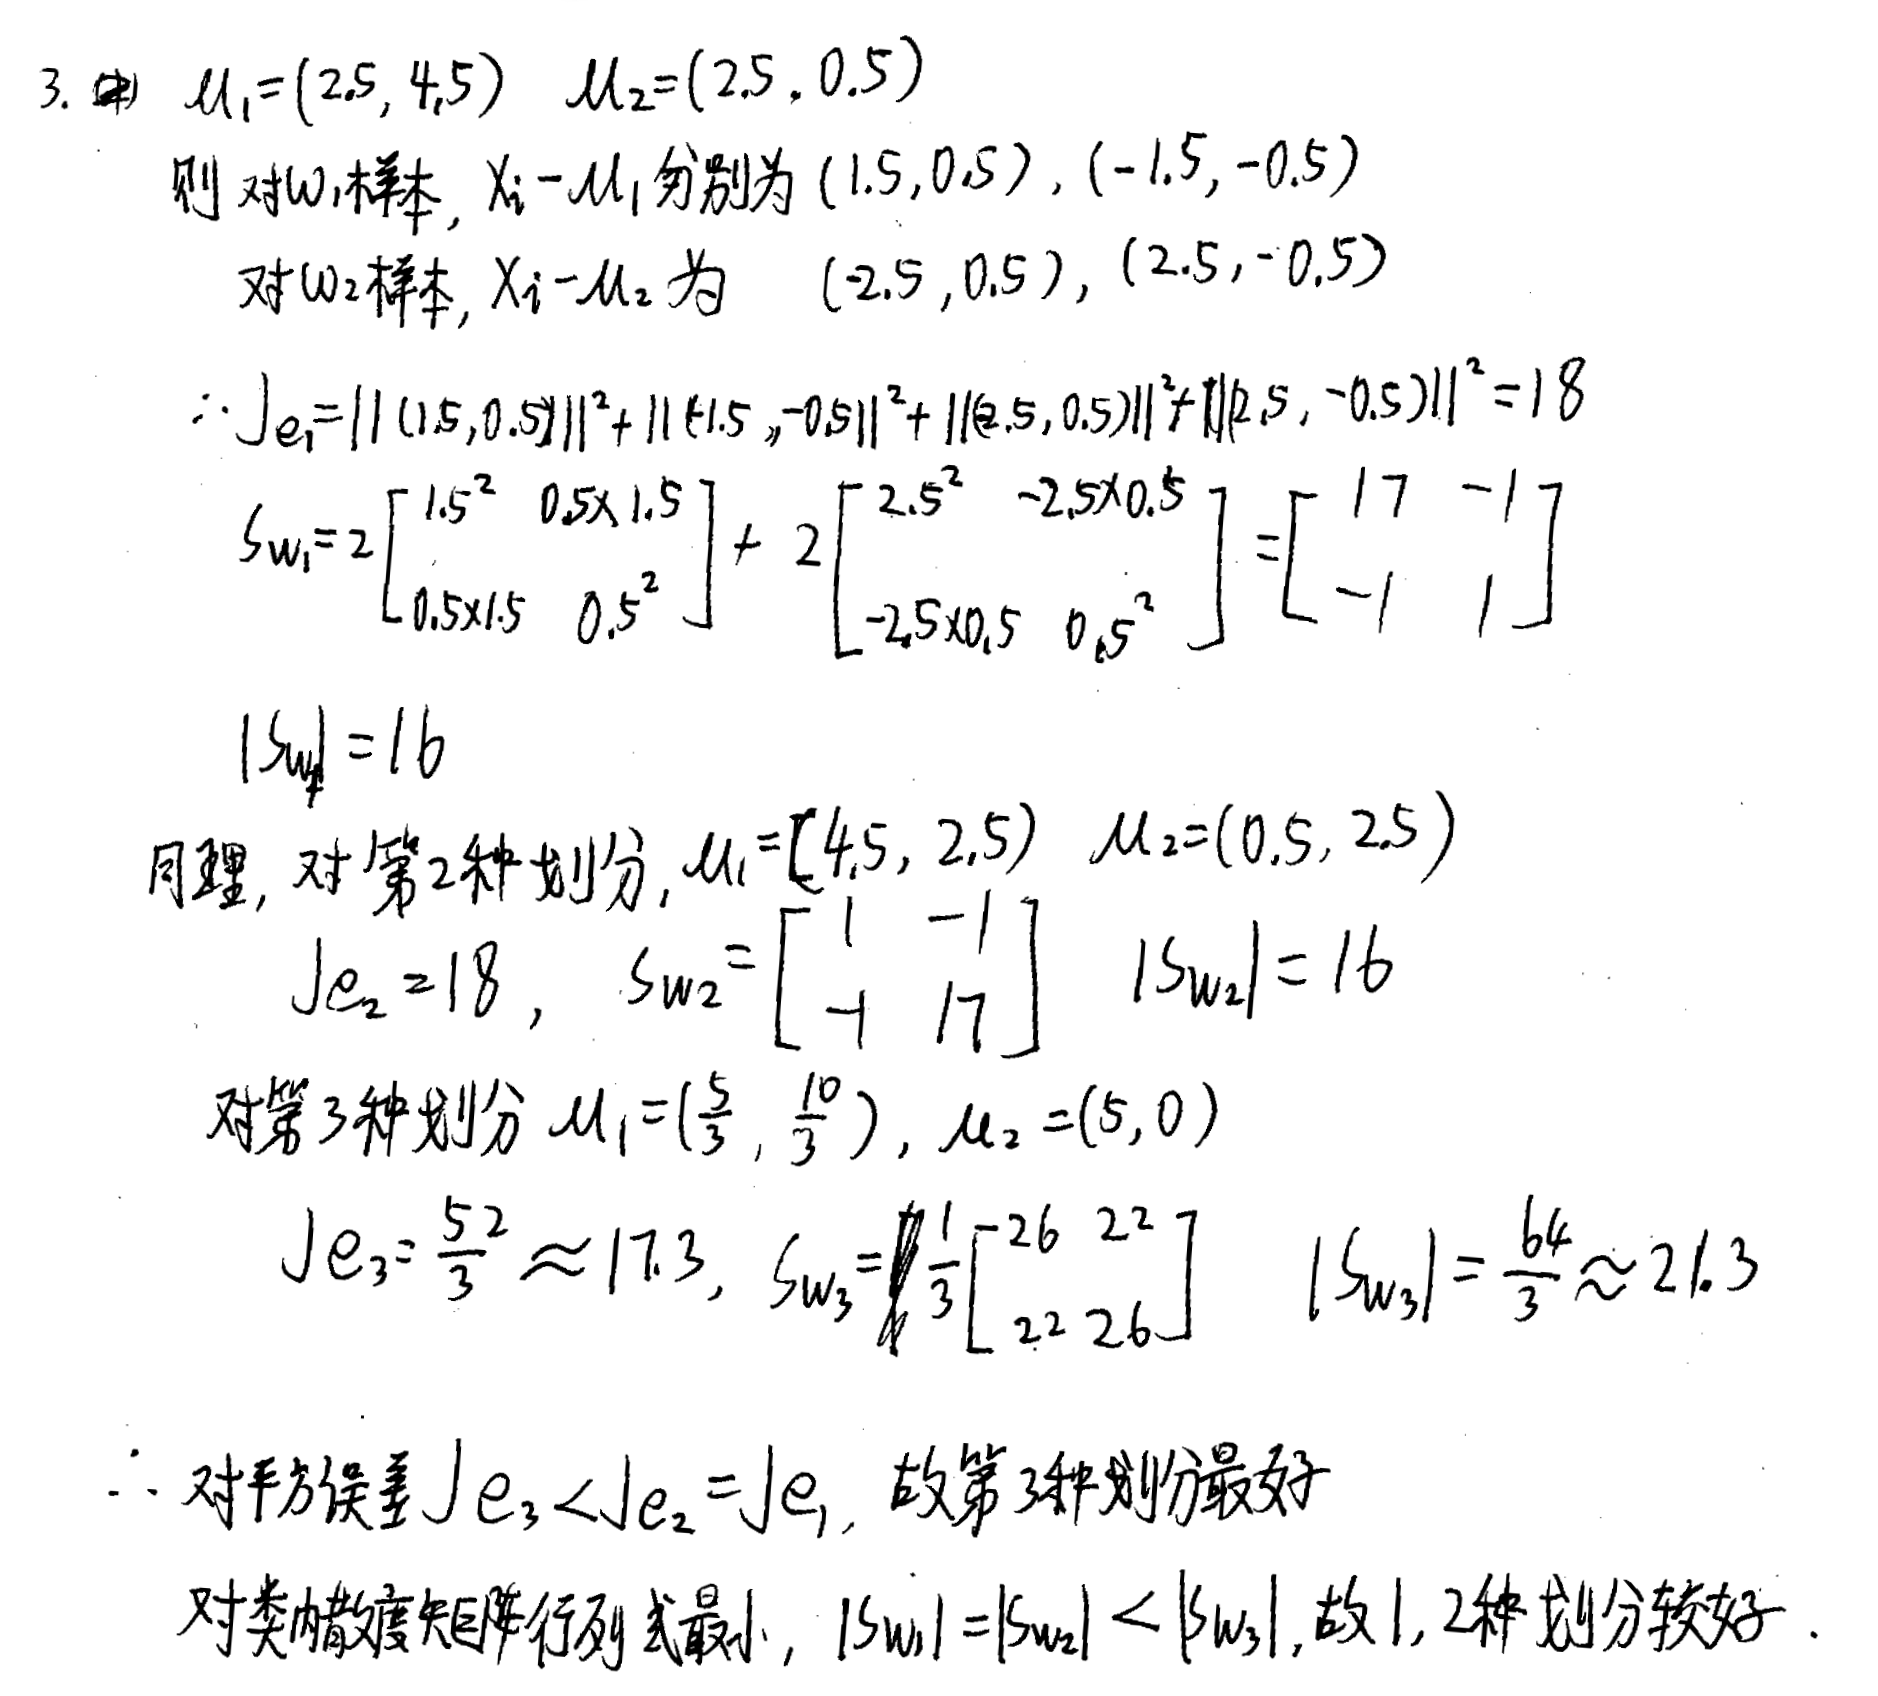
\includegraphics[scale=1.0]{P3.png}
    \end{figure}
    \section{Programming Problem 1}
    \subsection{Result}
    \begin{table}[h!]
            \centering            
            \begin{tabular}{c|*{2}{c}}
            \hline
$Clastur No.$ & $center$ & $Number of samples$  \\
\hline
$1$ & $200$ & $(5.93835690,  4.47548968)$  \\
$2$ & $201$ & $(5.47541305, -4.52601645)$  \\
$3$ & $200$ & $(1.02155866, -0.93527395)$  \\
$4$ & $199$ & $(1.07159471,  4.01702333)$  \\
$5$ & $200$ & $(9.00870491, -0.04025460)$  \\
            \hline            
            \end{tabular}
\end{table}

    \subsection{Code}
    \lstinputlisting[language=Python]{PP1.py}
    
    \section{Programming Problem 1}
    \subsection{Result}
    \begin{figure}[H]
        \centering
        %\includegraphics[scale=0.5]{PP1.png}
        \caption{Figure for Batch BP}
    \end{figure}
    \subsection{Code}
    \lstinputlisting[language=Python]{PP2.py}

\end{document}